\newcommand{\picwidth}{0.7\textwidth}

\section{Research Object Examples}
\label{sec:examples}

A number of exemplar Research Objects have been created. These
provide illustrative examples of how the model may be used to describe
aggregations of content. 

\subsection{Astrophysical Quantities}

This RO collects together several resources including input and output
datasets, scripts, web services and other documents. These relate to
various tasks and stages of the experiment including
\emph{gathering}, \emph{propagation} and \emph{comparison} with
intermediate results being passed from one stage to another. 

A screenshot of the RO within the RODL is shown in
Figure~\ref{fig:hyperleda}. This shows the conceptual view of the RO,
with folders containing Workflow Runs expanded.

\begin{figure}[h]
  \centering
  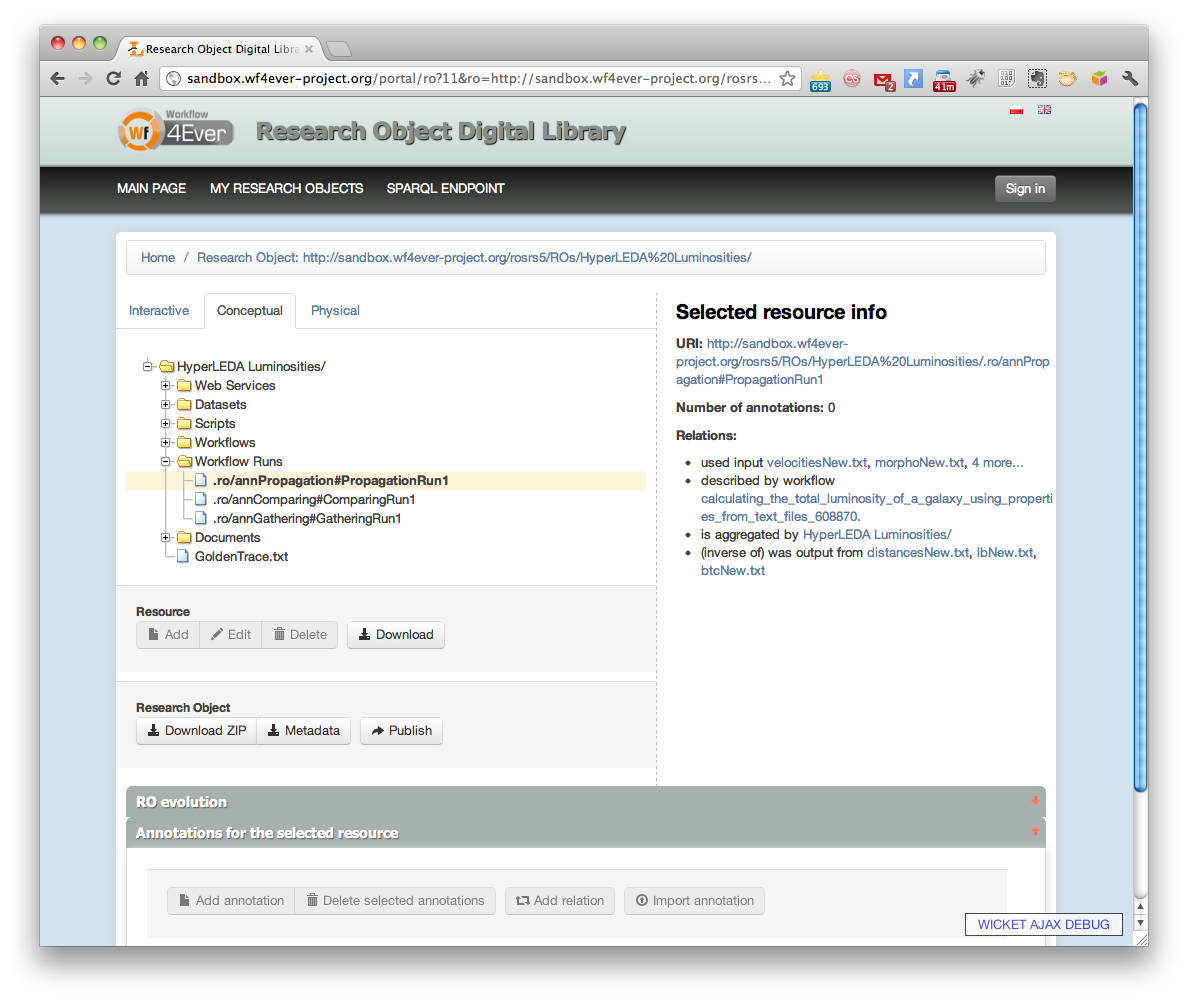
\includegraphics[width=\picwidth]{Figures/HyperLEDA}
  \caption{HyperLEDA Luminosities Example RO}
  \label{fig:hyperleda}
\end{figure}

We can see here the relationships between a particular workflow run
aggregated in the RO and its input, the workflow executed etc. These
relationships are described using the RO model vocabulary, and the
portal allows for export/publication of this metadata. 

The RO is available in the RODL
portal\footnote{\url{http://purl.org/net/wf4ever/ro/HyperLEDA_Luminosities}}

\subsection{InterProScan}

This is an example of an RO built around a workflow taken from
myExperiment. The workflow performs an InterProScan analysis of a
protein sequence using the EBI's\footnote{European Bioinformatics Institute} WSInterProScan service\footnote{\url{http://www.ebi.ac.uk/Tools/webservices/services/archive/pfa/wsinterproscan}}. The
workflow illustrates the issue of workflow \emph{decay} as it can no
longer be enacted. This is because the workflow involves EBI
asynchronous services that were suspended as the EBI changed the way
asynchronous services are handled. 

\begin{figure}[h]
  \centering
  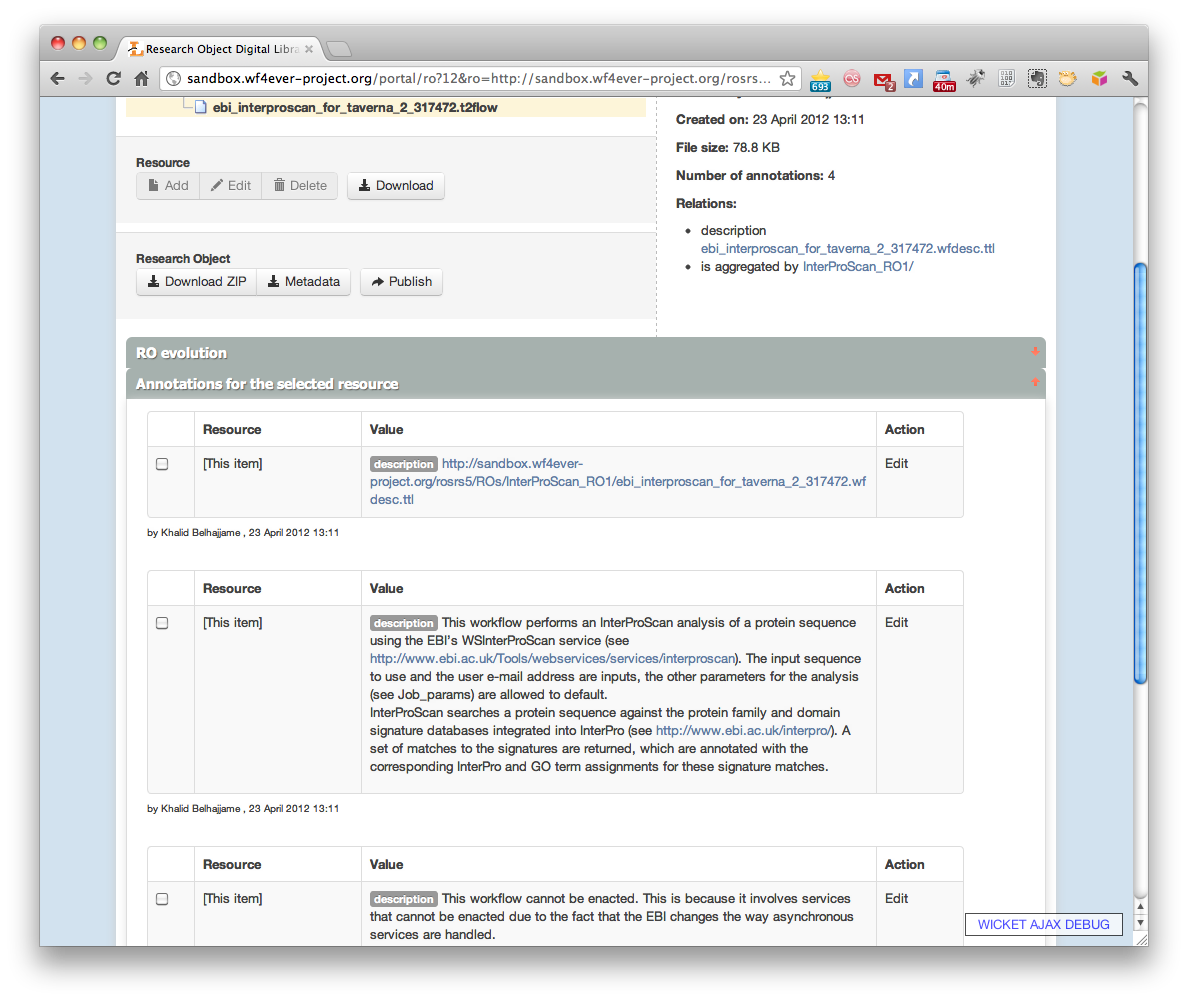
\includegraphics[width=\picwidth]{Figures/interpro}
  \caption{InterProScan Example RO}
  \label{fig:interpro}
\end{figure}

Again, a snapshot of the RO in RODL is shown in
Figure~\ref{fig:interpro}. Here, we can see annotation applied to the
workflow within the RO, in particular a description discussing the
problems with the workflow. 

The RO is available in the RODL portal\footnote{\url{http://purl.org/net/wf4ever/ro/InterProScan_RO1}}

\subsection{Repeatability and Reproducibility}

Two example ROs illustrate how different levels of information can be
recorded within the ROs in order to support a rerunning of an
experiment. Figure~\ref{fig:repeat}) includes a workflow (along with
its abstract description using the \textbf{wfdesc} ontology). In
Figure~\ref{fig:reproduce}, the RO also includes details of a workflow
execution or run, using the \textbf{wfprov} ontology.

\begin{figure}[h]
  \centering
  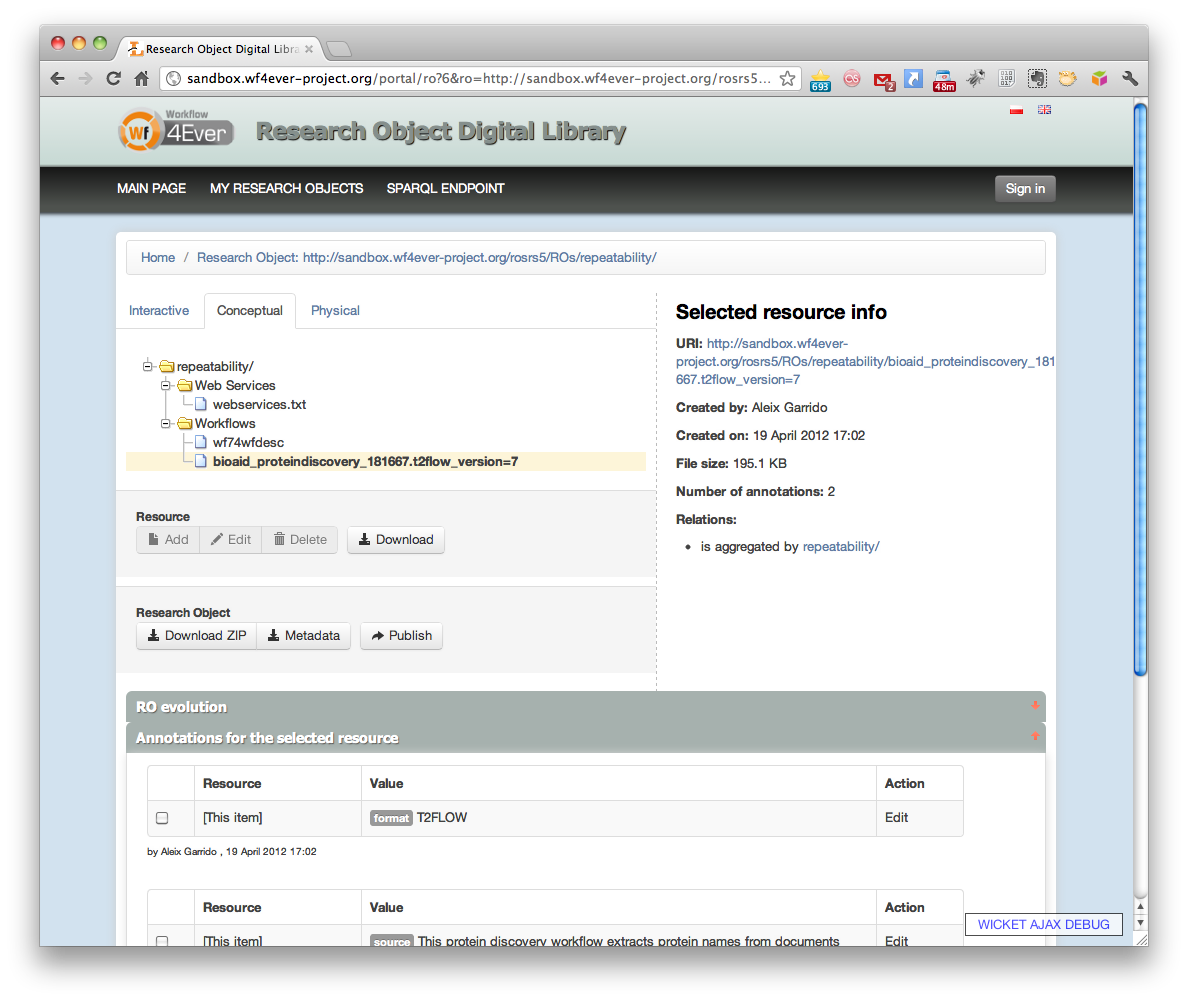
\includegraphics[width=\picwidth]{Figures/repeat}
 \caption{RO with Workflow description}
  \label{fig:repeat}
\end{figure}


\begin{figure}[h]
  \centering
  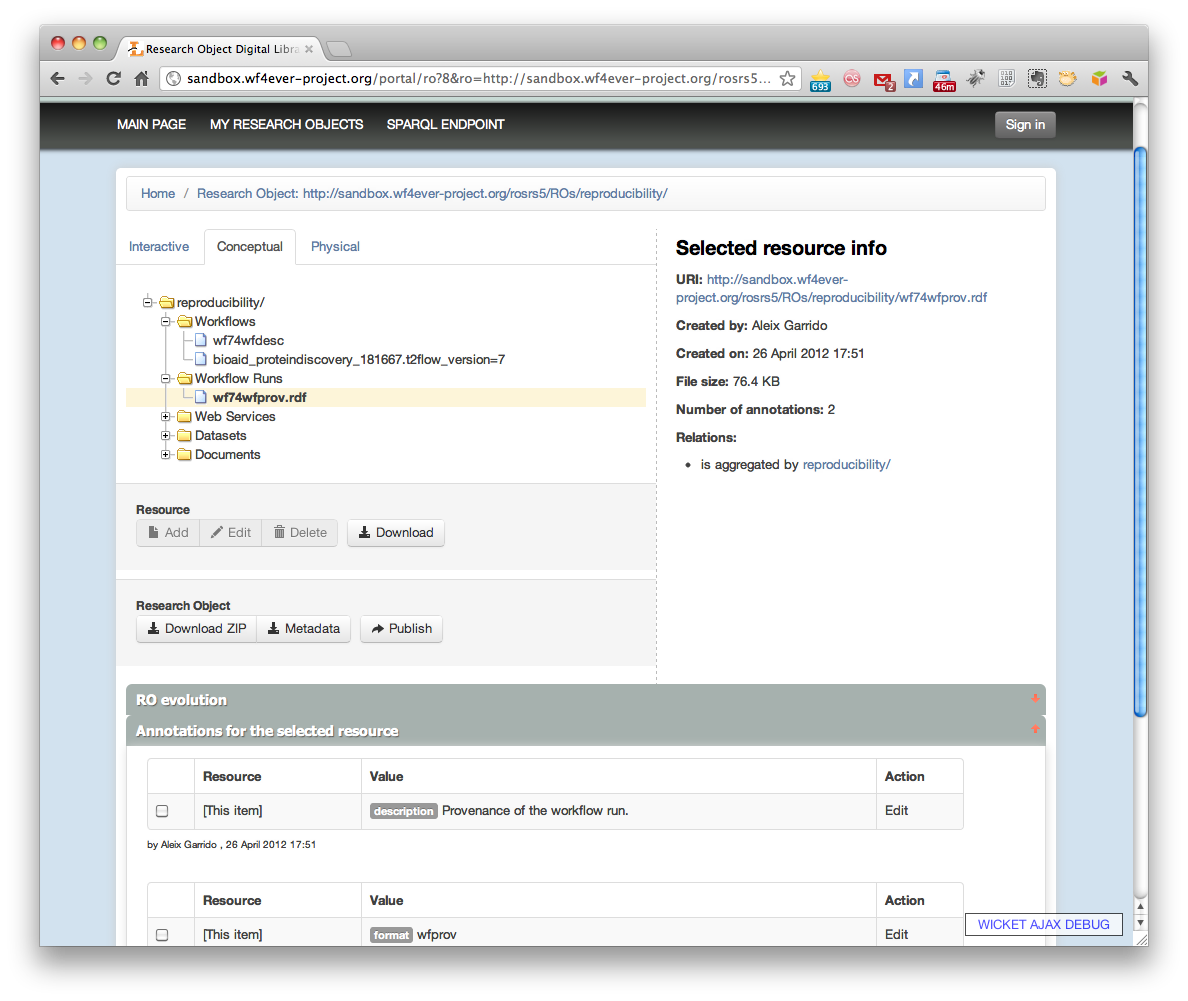
\includegraphics[width=\picwidth]{Figures/reproduce}
\caption{RO with Workflow provenance}
  \label{fig:reproduce}
\end{figure}


The ROs are available in the RODL
portal\footnote{\url{http://purl.org/net/wf4ever/ro/repeatability} and
  \url{http://purl.org/net/wf4ever/ro/reproducibility}}
